%-----------------------------------------------------------------------------%
\chapter{\babTiga}
%-----------------------------------------------------------------------------%
%\todo{tambahkan kata-kata pengantar bab 1 disini}
Penelitian ini bertujuan untuk mengevaluasi konfigurasi Hypervisor KVM yang disediakan secara langsung dalam konteks penggunaan Virtual Machine pada Apache Cloudstack. Tujuan utama adalah untuk memastikan bahwa Virtual Machine dapat mencapai kinerja yang optimal sesuai dengan spesifikasi sistem yang digunakan. Untuk mencapai tujuan ini, \saya akan melakukan penyesuaian konfigurasi atau tuning pada Hypervisor KVM dan kemudian membandingkannya dengan kondisi awal yang tidak mengalami tuning. Hasil pengujian akan dianalisis untuk menentukan apakah ada perbedaan signifikan dalam kinerja antara Hypervisor KVM yang telah dituning dengan yang belum dituning.

%-----------------------------------------------------------------------------%
\section{Tahapan Penelitian}
%-----------------------------------------------------------------------------%
\begin{figure}
	\centering
	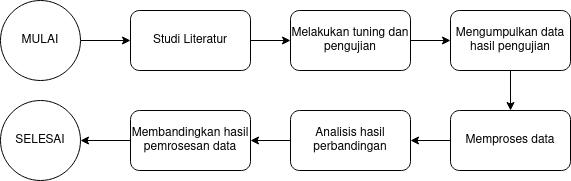
\includegraphics[width=1\textwidth]
	{assets/pics/tahapan-penelitian.png}
	\caption{Tahapan Penelitian}
	\label{fig:TahapanPenelitian}
\end{figure}

Penelitian ini akan dilakukan dalam beberapa tahap sesuai dengan diagram di gambar \ref{fig:TahapanPenelitian}. Tahap pertama melibatkan studi literatur untuk mengumpulkan semua informasi yang diperlukan untuk penelitian ini. Studi literatur ini penting karena memberikan dasar pengetahuan yang kuat tentang topik yang akan diteliti, memungkinkan \saya untuk memahami konteks dan kerangka kerja yang relevan.

Selanjutnya, penelitian melibatkan tuning terhadap Hypervisor KVM dan pengujian dilakukan dengan mengkompresi video menggunakan aplikasi Handbrake. Pengujian dengan Handbrake bertujuan untuk mengukur efisiensi dan kinerja Hypervisor KVM setelah tuning. Hasil pengujian Handbrake ini akan digunakan untuk membandingkan waktu kompresi video antara Hypervisor KVM yang tidak dituning dengan yang sudah dituning. Hasil dari perbandingan ini akan memberikan gambaran mengenai konfigurasi yang paling optimal dan sesuai, serta membantu dalam pemahaman lebih lanjut tentang pengaruh tuning terhadap performa Hypervisor KVM dalam konteks kompresi video.

%-----------------------------------------------------------------------------%
\section{Tuning Hypervisor KVM}
%-----------------------------------------------------------------------------%
Konfigurasi tuning yang dilakukan adalah dengan menambahkan parameter 

flag default host
\begin{verbatim}
	fpu vme de pse tsc msr pae mce cx8 apic sep mtrr pge mca cmov pat 
	pse36 clflush mmx fxsr sse sse2 ht syscall nx mmxext fxsr_opt pdpe1gb 
	rdtscp lm constant_tsc rep_good acc_power nopl nonstop_tsc cpuid 
	extd_apicid aperfmperf pni pclmulqdq monitor ssse3 fma cx16 sse4_1 
	sse4_2 movbe popcnt aes xsave avx f16c lahf_lm cmp_legacy svm extapic 
	cr8_legacy abm sse4a misalignsse 3dnowprefetch osvw ibs xop skinit wdt 
	lwp fma4 tce nodeid_msr tbm topoext perfctr_core perfctr_nb bpext ptsc 
	mwaitx cpb hw_pstate ssbd vmmcall fsgsbase bmi1 avx2 smep bmi2 xsaveopt 
	arat npt lbrv svm_lock nrip_save tsc_scale vmcb_clean flushbyasid 
	decodeassists pausefilter pfthreshold avic v_vmsave_vmload vgif 
	overflow_recov
\end{verbatim}


flag default kvm
\begin{verbatim}
	fpu de pse tsc msr pae mce cx8 apic sep mtrr pge mca cmov pat 
	pse36 clflush mmx fxsr sse sse2 syscall nx lm rep_good nopl 
	cpuid extd_apicid tsc_known_freq pni cx16 x2apic hypervisor 
	lahf_lm svm 3dnowprefetch vmmcall
\end{verbatim}

\begin{listing}[H]
	\begin{minted}{xml}
		<domain type='kvm'>
			<name>i-2-4-VM</name>
			<uuid>03704890-7c15-4f0a-bd11-4669a8424018</uuid>
			<description>Ubuntu 22.04 LTS</description>
			<memory unit='KiB'>1048576</memory>
			<cputune>
				<shares>1000</shares>
			</cputune>
			<os>
				<type arch='x86_64' machine='pc-i440fx-6.2'>
					hvm
				</type>
				<boot dev='cdrom'/>
				<boot dev='hd'/>
				<smbios mode='sysinfo'/>
			</os>
			<features>
				<acpi/>
				<apic/>
				<pae/>
			</features>
			<cpu mode='custom' match='exact' check='full'>
				<model fallback='forbid'>qemu64</model>
				<feature policy='require' name='x2apic'/>
				<feature policy='require' name='hypervisor'/>
				<feature policy='require' name='lahf_lm'/>
			</cpu>
			<disk type='file' device='cdrom'>
		</domain>
	\end{minted}
	\caption{Konfigurasi default dari KVM}
	\label{code:default_kvm_xml}
\end{listing}

\iffalse
%-----------------------------------------------------------------------------%
\section{Satu Persamaan}
%-----------------------------------------------------------------------------%

\noindent \begin{align}\label{eq:garis}
	\cfrac{y - y_{1}}{y_{2} - y_{1}} = 
	\cfrac{x - x_{1}}{x_{2} - x_{1}}
\end{align}

\equ~\ref{eq:garis} diatas adalah persamaan garis. 
\equ~\ref{eq:garis} dan \ref{eq:bola} sama-sama dibuat dengan perintah \bslash
align. 
Perintah ini juga dapat digunakan untuk menulis lebih dari satu persamaan. 

\noindent \begin{align}\label{eq:bola}
	\underbrace{|\overline{ab}|}_{\text{pada bola $|\overline{ab}| = r$}} 
		= \sqrt[2]{(x_{b} - x_{a})^{2} + (y_{b} - y_{a})^{2} + 
				\vert\vert(z_{b} - z_{a})^{2}}
\end{align}

%-----------------------------------------------------------------------------%
\section{Lebih dari Satu Persamaan}
\label{sec:multiEqu}
%-----------------------------------------------------------------------------%
\noindent \begin{align}\label{eq:matriks}	
	|\overline{a} * \overline{b}| &= |\overline{a}| |\overline{b}| \sin\theta 
		\\[0.2cm]
	\overline{a} * \overline{b} &=  
		\begin{array}{| c c c |}
			\hat{i} & x_{1} & x_{2} \\
			\hat{j} & y_{1} & y_{2} \\
			\hat{k} & z_{1} & z_{2} \\
		\end{array} \nonumber \\[0.2cm]
	&= \hat{i} \,
		\begin{array}{ | c c | }
			y_{1} & y_{2} \\
			z_{1} & z_{2} \\
		\end{array} 
	   + \hat{j} \,
		\begin{array}{ | c c | }
			z_{1} & z_{2} \\
			x_{1} & x_{2} \\
		\end{array} 
	   + \hat{k} \,	
		\begin{array}{ | c c | }
			x_{1} & x_{2} \\
			y_{1} & y_{2} \\
		\end{array}
		\nonumber
\end{align}

Pada \equ~\ref{eq:matriks} dapat dilihat beberapa baris menjadi satu bagian 
dari \equ~\ref{eq:matriks}. 
Sedangkan dibawah ini dapat dilihat bahwa dengan cara yang sama, \equ~
\ref{eq:gabungan1}, \ref{eq:gabungan2}, dan \ref{eq:gabungan3} memiliki nomor 
persamaannya masing-masing. 

\noindent \begin{align}\label{eq:gabungan1}	
	\int_{a}^{b} f(x)\, dx + \int_{b}^{c} f(x) \, dx = \int_{a}^{c} f(x) \, dx
		\\\label{eq:gabungan2}
	\lim_{x \to \infty} \frac{f(x)}{g(x)} = 0 \hspace{1cm} 
		\text{jika pangkat $f(x)$ $<$ pangkat $g(x)$} \\\label{eq:gabungan3}
	a^{m^{a \, ^{n}\log b }} = b^{\frac{m}{n}}
\end{align}
\fi
